\chapter{Introduction}

The internet, as we know it today, heavily relies on the use of the HTTP protocol. Not only is it
used by web browsers to download and otherwise interact with websites, it also serves as a transport
medium for use with REST web APIs or popular technologies such as gRPC and GraphQL\@.

Currently, the latest published version of the protocol is HTTP/2 defined in RFC 7540 from 2015.
HTTP/2 improved on its predecessor HTTP/1.1 by introducing features such as request multiplexing
over a single TCP connection, header compression and the server-push feature, allowing it to
significantly reduce loading times of web pages and generally improve the efficiency of the web.

However, HTTP/2 protocol performance is still limited in some scenarios and some limiting
factors can be traced to the TCP protocol used on the transport layer. Combination of request
multiplexing and TCP's guaranteed in-order delivery leads to a situation where the loss of a TCP
packet bearing data for one request will delay transmission of packets bearing data for other
requests. This problem is generally known as \textit{head-of-line blocking}.

Another area where HTTP/2 protocol can be improved is the connection establishment latency. For
security reasons, almost all web connections now use HTTPS instead of plain HTTP\@.
Establishment of HTTPS connection requires first establishing the TCP connection via the three-way
handshake, and then performing another handshake at the TLS protocol layer for negotiating
encryption. This process combined requires several round trips before the first packet with the
actual HTTP request can be sent.

The above mentioned and other problems are addressed in the HTTP/2's successor HTTP/3. At the time
of writing, the specification of HTTP/3 is still at the draft stage, but only small details of the
protocol are expected to change. HTTP/3 does not introduce new features at HTTP level, but instead
replaces the TLS and TCP protocols with a brand new UDP-based protocol named QUIC\@. Although QUIC
specification development is tied with that of HTTP/3, it is designed as a general-purpose transport
layer protocol that can be used for other higher application level protocols as well. The
relationships between protocols on HTTP/2 and HTTP/3 stacks are illustraded in
figure~\ref{fig:http2-vs-http3-stack}.

\begin{figure}[h]\label{fig:http2-vs-http3-stack}
  \centering
  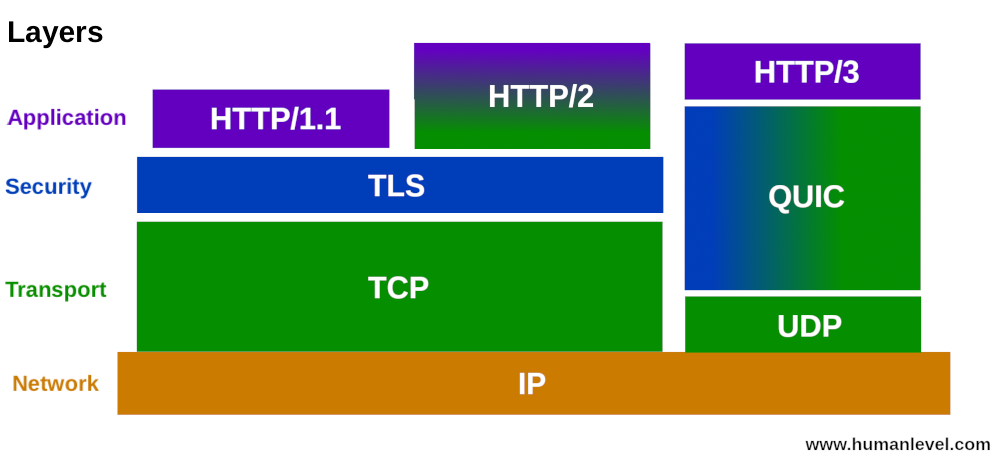
\includegraphics[width=\textwidth]{img/01-pile-http-protocol}
  \todo{Redraw this without HTTP/1.1 in inkscape}
  \caption{Comparison between HTTP/2 and HTTP/3 protocol stacks}
\end{figure}

The main improvements of QUIC over TCP+TLS can be summarized in following points:

\begin{itemize}
  \item \textit{Stream multiplexing} ---
    QUIC provides abstraction of multiple streams multiplexed on a single connection at the
    transport level. And because loss detection and retransmission is implemented at also the QUIC
    layer, rather than UDP, the protocol does not exhibit the \textit{head-of-line blocking} problem
    described previously.

  \item \textit{Faster connection establishment} ---
    QUIC intertwines TCP-like three-way-handshake and TLS 1.3 handshake together, requiring fewer
    round-trips to establish new connections and thus reducing latency. QUIC also supports TLS 1.3
    Zero Round Trip Time Resumption (a.k.a. 0-RTT) \todo{Explanation?:
    https://blog.cloudflare.com/introducing-0-rtt/}, allowing it to send user data with the very first
    packet.

  \item \textit{Always encrypted} ---
    Because TLS handshake is part of connection establishment, the QUIC connection is always
    encrypted. QUIC is therefore secure-by-default and no extra steps need to be taken by the
    application protocol to achieve security.

  \item \textit{Separating connection identification from peer's address} ---
    QUIC protocol identifies the connection using its ID rather than the peer's address. This
    feature is generally useful for mobile devices, which can often switch networks between Wi-Fi and
    mobile internet connection \todo{is it called GSM?}. With QUIC, these devices do not require
    reconnecting, but the connection can be migrated transparently to the application protocol.

    This feature also enables possible QUIC extensions like Multipath QUIC, which would allow
    simulataneous use of multiple network interfaces for a single connection to achieve greater
    throughput for a single connection. \todo{https://multipath-quic.org/}

\end{itemize}

Even though the QUIC specification is not yet finalized, there are multiple implementations
of the draft standard versions. Many of which are backed by big companies such as Cloudfare,
Facebook and Microsoft. These implementations are used to evaluate the protocol specification and
research improvements to the protocol.

Measurements on these implementations allow performance comparisons between HTTP/3 and HTTP/2. In
2015 the experimental implementation by the Chromium team showed a 3\% improvement in mean page load
time and 30\% less rebuffers when watching videos~\cite{Wilk2015}. Cloudfare launched HTTP/3 support
in April 2020 and has measured 12.4\% improvement in \textit{time to first byte}
metric~\cite{Tellakula2020}, demonstrating the promised reduced latency.

\section{Support for QUIC in \dotnet{}}

Microsoft's development team has long-term plans to provide full QUIC and HTTP/3 support in \dotnet{}.
In case of HTTP/3, the goal is that HTTP/3 be used by library classes such as \texttt{HttpClient},
completely transparent to the user. Since QUIC can be used to build other protocols as well, its
implementation will be publicly exposed, most likely via classes in the \texttt{System.Net.Quic}
namespace.

There has already been some work done on HTTP/3 and QUIC support. However, once it became clear that
the final specification for HTTP/3 and QUIC will not be ready in time for it to be implemented for
the upcoming \dotnet{} 5 release, the QUIC protocol API has been made internal and further work has
been postponed.

Current QUIC implementation in \dotnet{} is implemented as a wrapper around Microsoft's msquic
library\footnote{https://github.com/microsoft/msquic} written in C, which has been also recently
open-sourced. The library supports Windows and Linux operating systems, and its design is focused on
high-performance scenarios. Future versions of Windows will also ship msquic in Windows kernel in
the form of \texttt{msquic.sys} driver. At the time of writing, msquic library does not yet support
macOS platform.

In general, depending on a native library from \dotnet{} can be problematic and managed
implementation is often preferable for maintenance and portability reasons. In order to provide the
feature on all platforms supported by \dotnet{}, the native library in question must support at
least the same platforms as \dotnet{}. If some platform is not supported, but an alternative library
exists, separate versions of \dotnet{} source code need to be maintained for these platforms.
Example of such platform-specific code in \dotnet{} libraries is the support for cryptographic
(X509) certificates. On Windows, the implementation is backed by Windows CryptAPI (crypt32.dll), and
on Linux and macOS, the implementation is backed by OpenSSL\@. \todo{macOS impl needs to be
  fact-checked}

Another reason why managed implementation is preferred is that native libraries may use a threading
model which is not appropriate for the desired API in \dotnet{} code. This requires additional
overhead on the \dotnet{} side. Performance impact of the overhead may outweigh the performance
gained by using the native library. \todo{ask Ziki to check following sentences} An example is the
integration with the \textit{curl}\footnote{https://github.com/curl/curl} library, which was used
in the past to implement handlers for HTTP requests. For multiple reasons, performance problems
being one of them \todo{get specific issues links from KZ?}, handling HTTP/2 requests has been
reimplemented in managed code and curl was used only as a backup. The performance considerations may
be valid for msquic integration, because the msquic library uses an event-based interface, and
\dotnet{} QUIC API is based on the abstract \texttt{Stream} class.

In short, implementation of QUIC in managed \dotnet{} code can bring following benefits:

\todo{is this summary still necessary?}
\begin{itemize}
  \item \textit{Experimentability} ---
    It is easier to make changes to managed code, as opposed to changing native code, especially
    when making changes to the API\@.

  \item \textit{Portability/maintainability} ---
    There is a single source code for all platforms.

  \item \textit{Performance} ---
    Tailoring the library's implementation to the \dotnet{} threading model removes the overhead at
    the interop boundary. Also, no objects need to be pinned on the heap.
\end{itemize}

The reasons above motivated Microsoft developers to decide that it would be better to have managed
implementation of the QUIC protocol and avoid adding native dependencies. This thesis seeks to
create a partial implementation of QUIC, which could be used as the basis of the future official
\dotnet{} implementation. This implies that our implementation should be done in a separate
development branch of the \todo{fork of?} \dotnet{} runtime code
repository\footnote{https://github.com/dotnet/runtime}.

The design of the API for \dotnet{} QUIC implementation has been interrupted and further work has
been postponed to after the upcoming \dotnet{} 5 release. Because, designing of APIs for official
\dotnet{} libraries is a lengthy process requiring review and approval from senior engineers
maintaining the codebase, and because the current version of the API is sufficient for simple use
cases, this thesis will avoid making any changes to the API and implement it without modifications.
This will make our implementation a direct drop-in replacement of the previous msquic-based
implementation and will allow us to compare performance of the two implementations side by side.

Implementing the full QUIC specification is outside the scope of a master thesis. Fortunately, some
parts of the specification are concerned with aspects that need not come into effect for many
connections, and can be therefore omitted from our prototype implementation. For example, most QUIC
connections are not likely to use the connection migration feature. Because we do not expect readers
to be fully familiar with the QUIC protocol specification and all its features, we will present an
overview of the protocol in chapter 2 \todo{link} and defer selection of the actual protocol
features to be implemented to the beginning of the analysis in chapter 3 \todo{link}. The design of
the implementation, however, should be such that the rest of the specification can be implemented in
the future.

\todo{do we need an app for demonstration? Aren't perf\@. comparisons with msquic enough?}

In order to demonstrate that our implementation works in practice, we will use it to create a simple
fileserver application. The sole purpose of the application will be sending set of files from a
directory on the server to the client, utilizing the stream multiplexing feature of QUIC to transfer
individual files in separate streams. The application will be tested in a simulated network
environment, allowing us to show that our implementation works reasonably well even in presence of
network problems such as packet loss or packet reordering.

\todo{maybe a figure?

  1 --- client initiates connection.

  2 --- server pushes number of files on first streams and individual files on other streams.

  3 --- after receiving everything, connection is closed.

}

\section{Goals of this thesis}

The following list summarizes the goals of this thesis presented in previous section.

\begin{enumerate}
  \item Select and implement sufficient subset of QUIC specification to support basic data transfer.

  \item Use the implementation to replace the msquic based one in \dotnet{} runtime while preserving
    the same API\@.

  \item Write an example application using the QUIC API, demonstrating that the implemented QUIC
    subset is sufficient.

  \item Compare the performance of the new implementation with the previous msquic-based one.

\end{enumerate}
